\chapter{2002:Madhu Sudan}
\label{chap:sudan}
\begin{center}
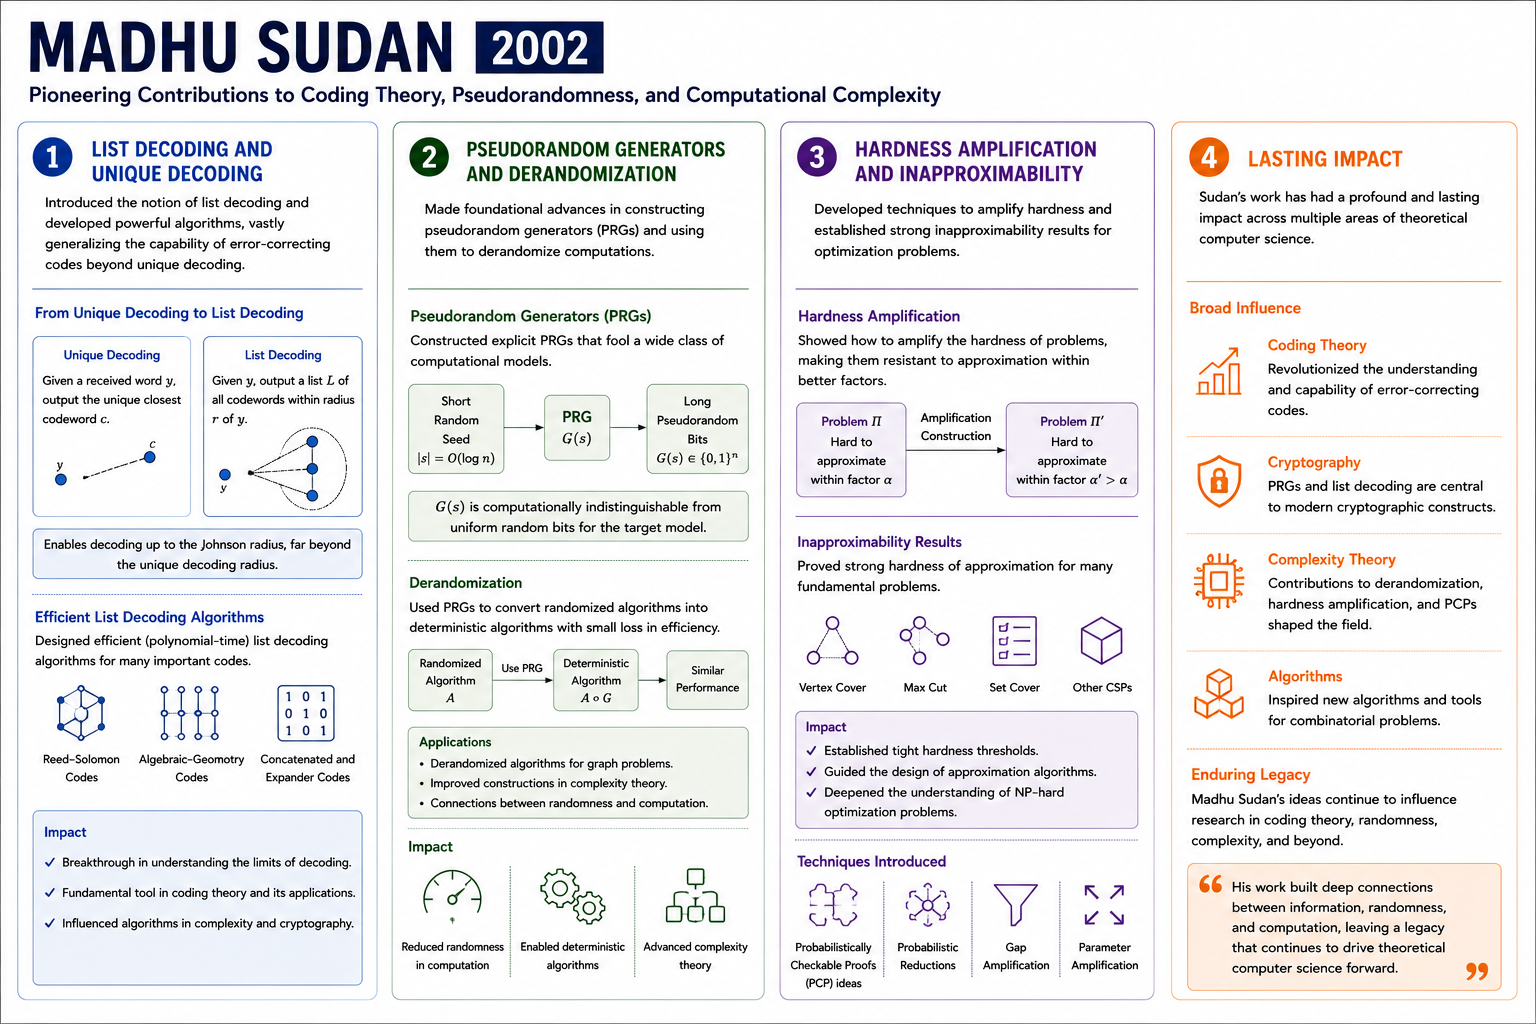
\includegraphics[width=\textwidth]{infographics/abacus6.png}
\end{center}
\targetchapterspacing
\index{Sudan, Madhu}

\booknote{The central habit in this chapter is to treat ambiguity as information: when the noise is heavy, the honest output of a decoder is a short list of every message that could explain what arrived, rather than one forced guess.}

\section{An Opening Story: Two Garbled Words, Four Plausible Messages}

A friend texts you a four-word sentence, and the channel scrambles two of the four words. What arrives is

\emph{MEET ?? OLD ??}

the question marks are unreadable words. The sentence could have been ``MEET AT OLD DOCK,'' ``MEET IN OLD TOWN,'' or ``MEET BY OLD MILL''---each explains exactly the fragments you received. A machine forced to print one sentence must guess---a coin flip that may send you to the wrong place. Two ruined words out of four outrun what cleverness can resolve from this message alone.

Yet the receiver is not helpless: the plausible sentences form a short list, and the true one is on it. A second text---``bring the fishing rod''---narrows the two together to one winner. The first message did not need to decide; it only had to keep every candidate alive until better evidence arrived. That division of labour, \emph{report the ambiguity now, resolve it later}, is the subject of this chapter, and Madhu Sudan's 2002 Rolf Nevanlinna Prize recognized the mathematics that made it efficient.

\section{The Problem}

An error-correcting code expands a message with redundancy so that noise can be repaired. A codeword is a valid expanded message; \emph{decoding} recovers the message from the corrupted string.

The classical contract is strict. If the code has \emph{minimum distance} $D$---the fewest positions in which two codewords differ---a decoder is guaranteed success exactly when the number of corrupted positions is at most $(D-1)/2$: inside that radius the received word is closer to its true codeword than to any other. This is \emph{unique decoding}: one received word, one answer, always right, provided the noise is mild.

Beyond radius $(D-1)/2$ the contract collapses: two codewords can be equidistant from the received word, so no rule always picks the true one. A unique decoder then guesses, and a guess destroys information. The hard question: must decoding stop there, or was the \emph{output contract} wrong?

\section{The World Before}

In 1950 Richard Hamming set the modern framework: a code is a set of strings with minimum distance $D$, and a decoder corrects up to $(D-1)/2$ errors by returning the nearest codeword. Hamming also priced codes---longer codewords buy more protection---so the subject could ask quantitative questions.

Reed--Solomon codes (1960) gave the framework its most beautiful example. Write the message as a polynomial $p(x)$ of degree at most $k$; the codeword is its values $p(a_1),\dots,p(a_n)$ at $n$ fixed points. Two distinct such polynomials agree in at most $k$ positions, so the minimum distance is $D=n-k$. Algebraic algorithms---Berlekamp--Welch, Berlekamp--Massey---decoded these codes in polynomial time all the way to the $(D-1)/2$ bound.

The barrier looked fundamental. A received word can sit halfway between two codewords, so no unique answer is always correct beyond half the minimum distance; this was read as ``heavy noise is hopeless.'' True for unique decoding, false for a different notion of ``the answer.'' In the late 1950s Elias and Wozencraft independently proposed \emph{list decoding}: return every codeword within the radius, not just one. The geometry was clear, but no efficient algorithm existed---trying every message is exponential---so it stayed exotic for thirty-five years.

One well-known fact was the seed: two distinct polynomials of degree at most $k$ agree in at most $k$ points, so agreement is sharp evidence. But organizing the search over all messages without checking them one by one---that nobody saw.

\section{The New Idea}

Sudan's insight begins with a question about what an answer should be. When several messages genuinely explain the received word, returning one candidate is not solving the problem; it hides the fact that the problem has several solutions. The correct output is the set of all explanations. \emph{Ambiguity can be managed mathematically: a short list is a better answer than a forced guess.}

The surprise is that this is not just philosophy; it makes heavy noise tractable. Sudan's 1997 algorithm rests on two counting arguments that expose every plausible message at once.

\emph{Unknowns versus equations.} Seek a nonzero bivariate polynomial $Q(x,y)$ vanishing at every received point $(a_i,b_i)$: one linear equation per point, in $Q$'s unknown coefficients. More coefficients than points means the system is under-determined, so a nonzero solution must exist. Two variables are essential: a univariate $Q(x)$ vanishing at $n$ points needs degree at least $n$, while a bivariate $Q(x,y)$ of small total degree has far more coefficients than $n$.

\emph{Roots versus degree.} If a message $p$ agrees with the received word in $t$ positions, $Q(x,p(x))$ is a univariate polynomial with $t$ roots. When $t$ exceeds its degree, $Q(x,p(x))\equiv0$, so $(y-p(x))$ divides $Q$: \emph{every sufficiently plausible message is a factor of $Q$}. Factoring $Q$ prints the list, which is short: at most one factor per degree of $y$.

Both counts succeed together. Sudan's algorithm then decodes in polynomial time up to roughly $n-\sqrt{2nk}$ errors, and Guruswami--Sudan improves this to roughly $n-\sqrt{n(k-1)}$ under the usual Reed--Solomon conventions; the unique-decoding radius is only about $(n-k)/2$. For small $k$ the list-decoding radii dwarf it, and the only price is a short list. The errors once declared ``impossible'' became routine.

\section{How It Works: Worked Examples}

\subsection{Four symbols, two errors, six honest answers}

Take a Reed--Solomon code with message polynomial $p(x)=2x+1$ of degree $k=1$, evaluated at $x=0,1,2,3$:
\[
(p(0),p(1),p(2),p(3))=(1,3,5,7).
\]
The minimum distance is $D=n-k=3$, so unique decoding corrects at most $(D-1)/2=1$ error. Suppose the received word is
\[
(1,0,0,7),
\]
the second and third symbols (values $3$ and $5$) corrupted. Two errors: unique decoding is beyond its guarantee.

List decoding returns every degree-1 polynomial agreeing with the received word in at least two positions. Since two distinct degree-1 polynomials agree in at most one point, each candidate is identified by the pair of positions where it agrees. From the points $(0,1),(1,0),(2,0),(3,7)$:
\begin{itemize}
\item $(0,1)$ and $(3,7)$: slope $(7-1)/(3-0)=2$, so $p(x)=2x+1$---the true message.
\item $(0,1)$ and $(1,0)$: slope $-1$, so $p(x)=1-x$.
\item $(1,0)$ and $(3,7)$: slope $7/2$, so $p(x)=\frac72(x-1)$.
\end{itemize}
Three more pairs give $p(x)=1-\frac12x$, $p(x)=0$, and $p(x)=7(x-2)$, for six candidates in total.

Check one: $p(0)=1$, $p(1)=0$, matching the received values. Six different messages explain the same evidence, the true one among them. A unique decoder might pick $p=1-x$ and lose the message; the list keeps $2x+1$ alive until later evidence selects it. (Reals are used for familiar arithmetic; over any field with at least four evaluation points the story is identical.)

\subsection{The bivariate polynomial in action}

Now use Sudan's machinery on the same points $(0,1),(1,0),(2,0),(3,7)$. A bivariate polynomial of total degree at most $2$ has $6$ coefficients:
\[
Q(x,y)=c_0+c_1x+c_2y+c_3x^2+c_4xy+c_5y^2.
\]
Requiring $Q(a_i,b_i)=0$ at the four points gives four homogeneous linear equations in six unknowns, so a nonzero solution must exist. One is
\[
Q(x,y)=7x^2+2y^2-21x-16y+14.
\]
Check: at $(0,1)$, $0+2-0-16+14=0$; at $(1,0)$, $7+0-21+0+14=0$; the other two cancel the same way. \emph{More unknown coefficients than constraints forces a nonzero $Q$}, and finding it is routine linear algebra.

Now substitute a candidate. For the true message $p=2x+1$,
\[
Q(x,2x+1)=15x^2-45x=15x(x-3),
\]
with roots $x=0,3$, exactly its agreement positions. For $p=1-x$,
\[
Q(x,1-x)=9x^2-9x=9x(x-1),
\]
roots at $x=0,1$. Here agreement $t=2$ equals the degree of $Q(x,p(x))$, so roots appear but are not forced; the forcing step needs the counting tilted. In Sudan's real regime---many points, $k\ll n$---a genuine candidate agrees in $t$ positions \emph{exceeding} that small degree; $Q(x,p(x))$ then has more roots than its degree permits, vanishes identically, and the candidate is a factor of $Q$. Factoring $Q$, or solving for its $y$-roots, prints the whole list in polynomial time.

\section{The Mathematics in Brief}

\emph{The agreement lemma.} Two distinct polynomials of degree at most $k$ agree in at most $k$ points. Why: their difference is a nonzero polynomial of degree at most $k$, which has at most $k$ roots.

\emph{Reed--Solomon geometry.} A message is a polynomial of degree at most $k$; its codeword is its $n$ values. Hence $D=n-k$ and the unique radius is $(D-1)/2=(n-k-1)/2$.

\emph{The list-decoding radius.} A Johnson-type bound says that for any code of distance $D=n-k$, agreement radius $\sqrt{nk}$ (about $n-\sqrt{nk}$ errors) yields only a polynomially bounded list. Sudan achieves this up to a constant factor ($n-2\sqrt{nk}$); Guruswami--Sudan reaches the Johnson bound exactly. The formula $\sqrt{nk}$ balances the counting: enough points for a sparse $Q$, yet enough agreements for $t$ to outrun the degree of $Q(x,p(x))$.

\emph{The $Q(x,y)$ method.} Choose $Q$ with more coefficients than points, so $Q(a_i,b_i)=0$ has a nonzero solution. A candidate agreeing in $t$ positions makes $Q(x,p(x))$ a degree-$(<t)$ polynomial with $t$ roots; it must vanish identically, so $p$ divides $Q$. With $B$ bounding the $y$-degree, the list has at most $B$ members. Every inequality has an algorithmic meaning: existence from linear algebra, extraction from factoring.

\emph{The proof-checking connection.} The same ``local evidence forces a global conclusion'' pattern powers probabilistically checkable proofs: encode a long proof, test a local relation at a few random positions, and let distance make a wrong proof fail most tests. Decoding and proof-checking are two faces of one idea: \emph{redundancy turns a few observations into a guarantee about the whole object}.

\section{Limits and Modern Views}

The list is polynomially bounded but not free: its precise size depends on the radius and interpolation parameters, and the field must supply $n$ distinct evaluation points, limiting block length; algebraic-geometry codes relax this and give the best known length--rate--distance tradeoffs. The Guruswami--Sudan refinement---weights and multiplicities in the interpolation---reaches the Johnson bound and extends to \emph{soft-decision decoding}, where each symbol carries a reliability score and weights favour trustworthy positions.

The PCP connection went beyond metaphor. These algebraic verification ideas became the engine of the PCP theorem---every proof can be encoded so that a verifier reading a constant number of random positions separates valid proofs from almost all invalid ones---and from it came hardness of approximation: problems like MAX-3SAT are hard even to approximate \cite{sudan-list,sudan-pcp}. Engineering inherited the same ideas: erasure coding (Reed--Solomon's descendant) protects RAID arrays and data centres, and list decoding appears in regenerating codes that repair a failed node from a few surviving blocks.

List decoding remains the honest statement of what decoding means. Heavy noise is not ``unsolvable''; it produces a short list, and shortening it to a winner is a job for side information, not the decoder. The field's slogan changed from ``correct the errors'' to ``know the plausible messages.''

\section{Exercises and Self-Study Guide}
\begin{enumerate}[label=\textbf{E\arabic*.}]
\item Prove the agreement lemma: two distinct polynomials of degree at most $k$ agree in at most $k$ points.
\hint{Subtract the two polynomials; a nonzero polynomial of degree at most $k$ has at most $k$ roots.}

\item Verify that $(1,0,0,7)$ is at Hamming distance $2$ from the codewords of both $p=2x+1$ and $p=1-x$, while the unique-decoding radius is $1$. Why must a unique decoder guess?
\hint{Write both codewords and count differing positions; a distance-$3$ code cannot tell them apart at radius $2$.}

\item Set up $Q(x,y)=c_0+c_1x+c_2y+c_3xy$ vanishing at the four received points and show it has only the zero solution; explain why adding $x^2$ and $y^2$ terms yields a nonzero one.
\hint{The first three points force $c_0=c_1=c_2=0$, the fourth forces $c_3=0$: four unknowns, four equations, no slack.}

\item A Reed--Solomon code has $n=100$ points and message degree $k=5$. Compare the unique-decoding radius with the list-decoding radius and state the agreement threshold for a guaranteed place on the list.
\hint{Unique radius $(n-k-1)/2\approx47$; list radius about $100-\sqrt{500}\approx78$ errors; the Johnson threshold is roughly $t>\sqrt{nk}\approx22$.}

\item Explain why $Q$ must have two variables; what goes wrong with a univariate $Q(x)$?
\hint{To vanish at $n$ points a univariate $Q$ needs degree at least $n$, so coefficients never beat the equations; the second variable carries the received value.}

\item The repetition code maps $0\mapsto000$, $1\mapsto111$. A local test reads two random positions and accepts if they match. Show it never rejects a valid codeword, and compute the rejection probability for $001$.
\hint{For $001$ the pairs $(0,0),(0,1),(0,1)$ disagree in two of three cases.}

\item Give an example where the worked-example list collapses to one message only after a second constraint, and name the constraint.
\hint{The received word cannot separate $2x+1$ from $1-x$; a second transmission revealing $p(1)=3$ leaves only $2x+1$.}
\end{enumerate}

\booknote{A final exercise in judgment: whenever a decoder is forced to return one answer, ask whether the ambiguity it suppresses is real. If two messages genuinely explain the same evidence, the honest output is the list; the winner should be chosen by side information, not by the decoder.}
\clearpage
